% Using the Revised NRSM template which meets the standard of NRSM & IEEE totally.
\documentclass[]{NRSMRev}

\NRSMsetup{
  stitle       = {Template for Two-Page Summary USNC-URSI National Radio Science Meeting},
  sauthor      = {Authors Name/s},
  subject      = {USNC-URSI National Radio Science Meeting},
  codeStyle    = {box}
}

% paper title
% can use linebreaks \\ within to get better formatting as desired
\title{Template for Two-Page Summary \\
USNC-URSI National Radio Science Meeting}

% author names and affiliations
% use a multiple column layout for up to three different
% affiliations
\author{\IEEEauthorblockN{Authors Name/s associated with 1st Affiliation}
\IEEEauthorblockA{line 1: dept. name (if applicable)\\
line 2: name of organization, acronyms acceptable\\
line 3: City, State/Province, Country\\
line 4: e-mail address if desired\\}
\and
\IEEEauthorblockN{Authors Name/s associated with 2nd Affiliation}
\IEEEauthorblockA{line 1: dept. name (if applicable)\\
line 2: name of organization, acronyms acceptable\\
line 3: City, State/Province, Country\\9444444444444787
line 4: e-mail address if desired}}

% conference papers do not typically use \thanks and this command
% is locked out in conference mode. If really needed, such as for
% the acknowledgment of grants, issue a \IEEEoverridecommandlockouts
% after \documentclass

% for over three affiliations, or if they all won't fit within the width
% of the page, use this alternative format:
%
%\author{\IEEEauthorblockN{Michael Shell\IEEEauthorrefmark{1},
%Homer Simpson\IEEEauthorrefmark{2},
%James Kirk\IEEEauthorrefmark{3},
%Montgomery Scott\IEEEauthorrefmark{3} and
%Eldon Tyrell\IEEEauthorrefmark{4}}
%\IEEEauthorblockA{\IEEEauthorrefmark{1}School of Electrical and Computer Engineering\\
%Georgia Institute of Technology,
%Atlanta, Georgia 30332--0250\\ Email: see http://www.michaelshell.org/contact.html}
%\IEEEauthorblockA{\IEEEauthorrefmark{2}Twentieth Century Fox, Springfield, USA\\
%Email: homer@thesimpsons.com}
%\IEEEauthorblockA{\IEEEauthorrefmark{3}Starfleet Academy, San Francisco, California 96678-2391\\
%Telephone: (800) 555--1212, Fax: (888) 555--1212}
%\IEEEauthorblockA{\IEEEauthorrefmark{4}Tyrell Inc., 123 Replicant Street, Los Angeles, California 90210--4321}}

% use for special paper notices
%\IEEEspecialpapernotice{(Invited Paper)}

\begin{document}

% make the title area
\maketitle

\begin{abstract}
%\boldmath
Please include a brief abstract here. The abstract should be limited to 50-200 words and should concisely state what was done, how it was done, principal results, and their significance.
\end{abstract}
% IEEEtran.cls defaults to using nonbold math in the Abstract.
% This preserves the distinction between vectors and scalars. However,
% if the conference you are submitting to favors bold math in the abstract,
% then you can use LaTeX's standard command \boldmath at the very start
% of the abstract to achieve this. Many IEEE journals/conferences frown on
% math in the abstract anyway.

% no keywords

% For peer review papers, you can put extra information on the cover
% page as needed:
% \ifCLASSOPTIONpeerreview
% \begin{center} \bfseries EDICS Category: 3-BBND \end{center}
% \fi
%
% For peerreview papers, this IEEEtran command inserts a page break and
% creates the second title. It will be ignored for other modes.
\IEEEpeerreviewmaketitle



\section{Introduction}
This LaTeX template provides authors with most of the formatting specifications (e.g. margins, column widths, line spacing, and text fonts) needed for preparing electronic versions of their papers. Please do not alter any of the formatting in this template when you prepare your paper.

\section{Preparing Your Paper}
Summary papers at the National Radio Science Meeting are limited to two pages. Any submitted paper that exceeds this limit will be rejected.  However, it is also important that your summary substantially fills up both of the two pages. If the summary is too short, it will also be rejected. The page format is two-column, as illustrated here.  Do not add any kind of pagination anywhere in the paper. Do not manually number the headings - the template will do that for you.

Please take note of the following items when preparing your paper:


\subsection{Authors and Affiliations}
The template is designed so that author affiliations are not repeated each time for multiple authors of the same affiliation. Please keep your affiliations as succinct as possible (for example, do not differentiate among departments of the same organization). This template was designed for two affiliations, but can be customized for fewer or more as described below.

\begin{enumerate}
\item For author/s of only one affiliation: Add the name of all authors inside the brackets in the first ``$\backslash$IEEEauthorblockN\{...\}'' block and use only one ``$\backslash$IEEEauthorblockA\{...\}" block after that.
\item For author/s of more than two affiliations: Add the name of all authors affiliated with the first affiliation to the first ``$\backslash$IEEEauthorblockN\{...\}" block. Identify the affiliation in the  ``$\backslash$IEEEauthorblockA\{...\}" that comes after that. Repeat this process for up to three different affiliations.
\end{enumerate}

\subsection{Headings}
Primary section headings within the paper are enumerated by Roman numerals and are centered above the text.  Secondary section headings are enumerated by capital letters followed by periods (``A.", ``B.", etc.) and are flush left above their sections. The first letter of each word is capitalized. Tertiary section headings are enumerated by Arabic numerals followed by a parenthesis. They are indented, run into the text in their sections, and are followed by a colon.

\subsection{Equations}
All equations should be labeled in consecutive numerical order. Equation numbers, within parentheses, should be aligned on the right side of the column, as in (1), using a right tab stop. Punctuate equations with commas or periods when they are part of a sentence, as in

\begin{equation} \label{eq:1}
\alpha+\beta=\chi.
\end{equation}
	            	
Be sure that the symbols in your equation have been defined before or immediately following the equation. Use ``\eqref{eq:1}", not ``Eq. \eqref{eq:1}" or ``equation \eqref{eq:1}", except at the beginning of a sentence: ``Equation \eqref{eq:1} is ..."

\subsection{Figures and Tables}
Place each figure and table within the width of a single column, as in \autoref{Fig1Label} and \autoref{Table1Label} below. (Please look at the Word version of the template to actually see Fig. 1.) Large figures and tables may span across both columns. Figure captions should be below the figures. Table headings should appear above the tables (note the capitalization). Insert figures and tables after they are cited in the text. It is helpful to the reader if your captions, when read in succession, form a quick summary of your paper so as to attract the interest of your target audience. Make sure your graphs and figures still make sense when printed entirely in black and white. If possible, it is preferred to label multiple curves directly rather than using tiny data markers and including a complicated legend look-up table. Make sure you use san-serif fonts large enough to be read easily when printed. Do not reference figures as ``Figure 1'' or ``Fig-1''.

Here is an example of referring figure: \autoref{Fig1Label}.

Here is another example of referring table: \autoref{Table1Label}.

Here is the third example of a footnote\footnote{See here to check the footnote.}.

\begin{figure}[h]
  \centering
  \noindent
  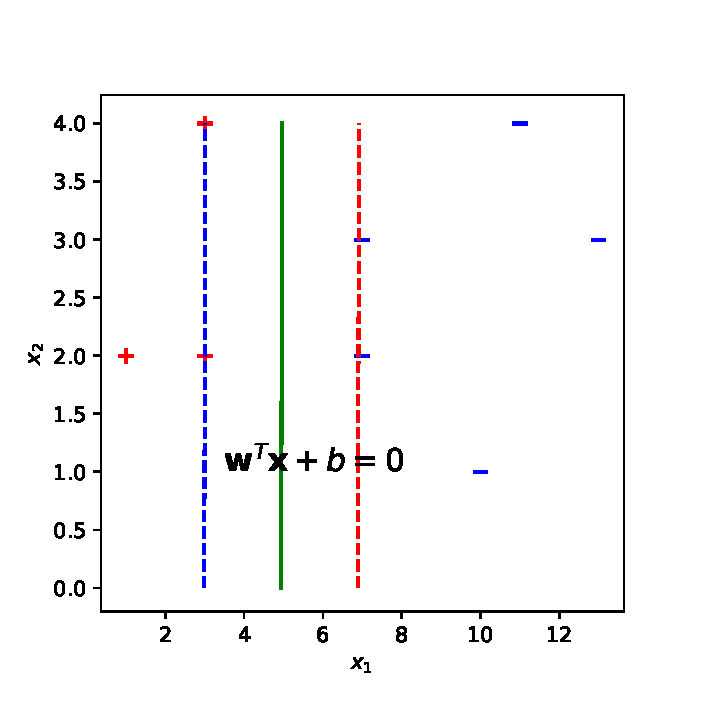
\includegraphics[width=1.5in]{pic-ex}
  \DeclareGraphicsExtensions.
  \caption{Example of a figure caption.}
  \label{Fig1Label}
\end{figure}

\begin{table}[h] 
  \centering
  \caption{Example of a table heading.}
  \begin{tabular}{|m{0.24\columnwidth}<{\centering}|m{0.24\columnwidth}<{\centering}|m{0.24\columnwidth}<{\centering}|}
    \hline
    Table Column Head 1 & Table Column Head 2 & Table Column Head 3\\
    \hline
    Item 4 & Item 5 & Item 6\\
    \hline
    Item 7 & Item 8 & Item 9\\
    \hline
  \end{tabular}
  \label{Table1Label}
\end{table}

\subsection{Abbreviations and Acronyms}
Always define technical abbreviations and acronyms the first time you use them in the text, no matter how simple they are, even if you have already defined them in the abstract. Abbreviations such as ``e.g.'' and ``i.e.'' are used without definition, but don’t forget that ``e.g.'' means ``for example'' and ``i.e.'' means ``in other words''. Do not confuse the two. Do not define (or re-define!) standard IEEE abbreviations for units.

\subsection{Units and Numbers}
The International System of Units (SI units) is used for use in IEEE publications. Unit symbols should be used with measured quantities, e.g., 1 mm, but not when unit names are used in text without quantities, e.g., ``a few millimeters." Use a zero before decimal points: ``0.25", not ``.25". Include a space between the number and the unit label when used as a noun. Replace the space with a hyphen when used as an adjective. For example, ``The 10-GHz antennas now operate at 9.8 GHz.'' The hyphen makes it clear that we are specifying frequency and not the number of antennas.

\subsection{References}
All references should be labeled in consecutive numerical order \cite{IEEEhowto:eason, IEEEhowto:maxwell, IEEEhowto:doe}. When citing references within the text, refer simply to the reference number enclosed by square brackets, as in \cite{IEEEhowto:eason}.  Do not use ``Ref. [1]" or ``reference [1]" except at the beginning of a sentence: ``Reference [1] was the first..." Note that an ``en-dash'', not a hyphen, should be used between numbers to indicate a range of numbers, as in the beginning of this paragraph. For example, write ``pp. 1--4'', not ``pp. 1-4''. Note the space between ``pp.'' and the page numbers.

A numbered list of references must be provided at the end of the paper. The list should be arranged in the order of citation in text, not in alphabetical order. Each reference should be given a unique reference number. Do not list references that are not cited in the text. Include all authors' names on a paper in the reference list; do not use ``et al.". Papers that have not been published, even if they have been submitted for publication, are cited as ``unpublished" \cite{IEEEhowto:doe}. Papers that have been accepted for publication are cited as ``in press". Capitalize only the first word in a paper title except for proper nouns and element symbols.

\subsection{Style Issues}
For detailed information on paper preparation, we highly recommend exploring the IEEE Author Digital Toolbox,
\url{http://www.ieee.org/publications_standards/publications/authors/authors_journals.html}. In particular, download and read the
IEEE Style Manual. View the material on figure preparation. We also recommend submitting your paper to the IEEE
Reference Preparation Assistant to verify the correctness of your references. If English is a second language, please
consider having a native English speaker proof read your paper. Fee based professional editing services are available at the
above link.

Careful attention to these matters results in a polished and professional appearance, imparting a first impression to your
prospective reader that is simply priceless.

% use section* for acknowledgement
\section*{ACKNOWLEDGEMENT}
An acknowledgement statement, if applicable, goes here. This section head is not numbered and is always singular, i.e., never ``Acknowledgements''.


% An example of a floating figure using the graphicx package.
% Note that \label must occur AFTER (or within) \caption.
% For figures, \caption should occur after the \includegraphics.
% Note that IEEEtran v1.7 and later has special internal code that
% is designed to preserve the operation of \label within \caption
% even when the captionsoff option is in effect. However, because
% of issues like this, it may be the safest practice to put all your
% \label just after \caption rather than within \caption{}.
%
% Reminder: the "draftcls" or "draftclsnofoot", not "draft", class
% option should be used if it is desired that the figures are to be
% displayed while in draft mode.
%
%\begin{figure}[!t]
%\centering
%\includegraphics[width=2.5in]{myfigure}
% where an .eps filename suffix will be assumed under latex,
% and a .pdf suffix will be assumed for pdflatex; or what has been declared
% via \DeclareGraphicsExtensions.
%\caption{Simulation Results}
%\label{fig_sim}
%\end{figure}

% Note that IEEE typically puts floats only at the top, even when this
% results in a large percentage of a column being occupied by floats.


% An example of a double column floating figure using two subfigures.
% (The subfig.sty package must be loaded for this to work.)
% The subfigure \label commands are set within each subfloat command, the
% \label for the overall figure must come after \caption.
% \hfil must be used as a separator to get equal spacing.
% The subfigure.sty package works much the same way, except \subfigure is
% used instead of \subfloat.
%
%\begin{figure*}[!t]
%\centerline{\subfloat[Case I]\includegraphics[width=2.5in]{subfigcase1}%
%\label{fig_first_case}}
%\hfil
%\subfloat[Case II]{\includegraphics[width=2.5in]{subfigcase2}%
%\label{fig_second_case}}}
%\caption{Simulation results}
%\label{fig_sim}
%\end{figure*}
%
% Note that often IEEE papers with subfigures do not employ subfigure
% captions (using the optional argument to \subfloat), but instead will
% reference/describe all of them (a), (b), etc., within the main caption.


% An example of a floating table. Note that, for IEEE style tables, the
% \caption command should come BEFORE the table. Table text will default to
% \footnotesize as IEEE normally uses this smaller font for tables.
% The \label must come after \caption as always.
%
%\begin{table}[!t]
%% increase table row spacing, adjust to taste
%\renewcommand{\arraystretch}{1.3}
% if using array.sty, it might be a good idea to tweak the value of
% \extrarowheight as needed to properly center the text within the cells
%\caption{An Example of a Table}
%\label{table_example}
%\centering
%% Some packages, such as MDW tools, offer better commands for making tables
%% than the plain LaTeX2e tabular which is used here.
%\begin{tabular}{|c||c|}
%\hline
%One & Two\\
%\hline
%Three & Four\\
%\hline
%\end{tabular}
%\end{table}


% Note that IEEE does not put floats in the very first column - or typically
% anywhere on the first page for that matter. Also, in-text middle ("here")
% positioning is not used. Most IEEE journals/conferences use top floats
% exclusively. Note that, LaTeX2e, unlike IEEE journals/conferences, places
% footnotes above bottom floats. This can be corrected via the \fnbelowfloat
% command of the stfloats package.






% conference papers do not normally have an appendix









% trigger a \newpage just before the given reference
% number - used to balance the columns on the last page
% adjust value as needed - may need to be readjusted if
% the document is modified later
%\IEEEtriggeratref{8}
% The "triggered" command can be changed if desired:
%\IEEEtriggercmd{\enlargethispage{-5in}}

% references section

% can use a bibliography generated by BibTeX as a .bbl file
% BibTeX documentation can be easily obtained at:
% http://www.ctan.org/tex-archive/biblio/bibtex/contrib/doc/
% The IEEEtran BibTeX style support page is at:
% http://www.michaelshell.org/tex/ieeetran/bibtex/
%\bibliographystyle{IEEEtran}
% argument is your BibTeX string definitions and bibliography database(s)
%\bibliography{IEEEabrv,../bib/paper}
%
% <OR> manually copy in the resultant .bbl file
% set second argument of \begin to the number of references
% (used to reserve space for the reference number labels box)
\begin{thebibliography}{1}


\bibitem{IEEEhowto:eason}
G. Eason, B. Noble, and I. N. Sneddon, ``On certain integrals of Lipschitz-Hankel type involving products of Bessel functions'', \emph{Phil. Trans. Roy. Soc. London}, vol. A247, pp. 529--551, April 1955.

\bibitem{IEEEhowto:maxwell}
J. Clerk Maxwell, \emph{A Treatise on Electricity and Magnetism, 3rd ed., vol. 2}. Oxford: Clarendon, 1892, pp. 68--73.

\bibitem{IEEEhowto:doe}
J. Doe, ``Title of paper if known'', unpublished. 
\end{thebibliography}




% that's all folks
\end{document}


